\documentclass[11pt]{article}

% ---------------------------------------------------------------------------
%  East Africa AI-rainfall benchmark -- pipeline overview
%  Standalone, single-file article. Compiles with pdflatex (needs TikZ).
% ---------------------------------------------------------------------------

\usepackage[margin=1in]{geometry}
\usepackage{amsmath,amssymb}
\usepackage{booktabs}
\usepackage{array}
\usepackage{siunitx}
\usepackage{xcolor}
\usepackage{enumitem}
\usepackage{tikz}
\usetikzlibrary{arrows.meta,positioning,fit,backgrounds,shapes.geometric,calc}
\usepackage[hidelinks]{hyperref}

% --- colours reused in the flow diagram -----------------------------------
\definecolor{cData}{HTML}{2E6E9E}
\definecolor{cModel}{HTML}{B5651D}
\definecolor{cPost}{HTML}{2E7D32}
\definecolor{cVerif}{HTML}{6A1B9A}
\definecolor{cBox}{HTML}{F5F5F0}

\newcommand{\code}[1]{\texttt{\small #1}}
\newcommand{\mmday}{mm\,day$^{-1}$}

\title{\vspace{-1.5em}A Reproducible Benchmark of AI Weather Models for
Daily Rainfall over East Africa:\\ Pipeline Overview and Experimental Setup}
\author{}
\date{}

\begin{document}
\maketitle
\vspace{-3em}

% ===========================================================================
\section{Introduction and motivation}
% ===========================================================================

Data-driven weather models --- graph neural networks, neural operators,
diffusion ensembles, and differentiable hybrid solvers --- now match or exceed
operational numerical weather prediction on many upper-air and surface fields at
a tiny fraction of the inference cost. Their skill for \emph{precipitation},
however, remains the least well characterised of their outputs: rainfall is
intermittent, heavy-tailed, and only weakly constrained by the reanalysis
targets these models are trained on. It is also the variable of greatest
societal consequence in the tropics. This pipeline was built to answer a
specific, operationally framed question with a single reproducible workflow:
\emph{do modern AI forecast systems add skill over a strong climatological
baseline for daily rainfall over East Africa, and if so at which lead times,
seasons, and rainfall intensities?}

East Africa is a deliberate and demanding choice of testbed. The Greater Horn
region has a bimodal rainfall regime --- the March--May ``long rains'' and the
October--December ``short rains'' --- driven by the migration of the ITCZ and
modulated by the Indian Ocean Dipole and ENSO, and is subject to recurrent,
high-impact flood and drought episodes. It is convectively dominated, so daily
rainfall has strong sub-grid structure; it is topographically complex; and it is
\emph{data sparse}, with few assimilated surface gauges, which both degrades the
reanalysis used to initialise the models and complicates verification. A region
where the training signal is weakest is precisely where the value of physical
constraints, ensemble calibration, and architecture choice can be
distinguished. The benchmark is intentionally self-contained: every input ---
model checkpoints, ERA5 initial conditions, and observational references --- is
public, and all inference is driven by one entry point that writes a common,
model-agnostic output format, so that any model or reference can be added
without touching the scoring code.

% ===========================================================================
\section{Meaning of ``2024''}
% ===========================================================================

Throughout this document and the codebase, \textbf{``2024'' denotes the forecast
\emph{initialization} period}, not a single case study. Inference is launched
(\code{run\_inference.sh}, \code{run\_inference\_parallel.sh},
\code{run\_neuralgcm.sh}) over initialization dates
\code{--start 2024-01-01 --end 2024-12-24}, i.e.\ one cold-start forecast per
calendar day, \num{359} initializations in total. The last initialization is
24~December so that a 7-day forecast still verifies within the same calendar
frame. \textbf{The verification/evaluation window is derived from these
initializations}: a forecast initialized on date $t$ is scored on its
\emph{valid} date $t+\ell$ for each lead $\ell\in\{1,3,5,7\}$~days, so the valid
dates being evaluated run from 2~January~2024 through the first week of
January~2025 (for the longest lead of the final initializations). The
verification driver takes its own \code{--start/--end/--obs-end} window and can
be pointed at the full year or at a single season.

% ===========================================================================
\section{Pipeline structure and data flow}
% ===========================================================================

The pipeline has two decoupled stages joined by a single on-disk contract.

\paragraph{Stage 1 --- inference (\code{benchmark\_ea/run.py}).}
A model-agnostic runner iterates a set of adapters over the initialization date
range and writes, per model and per initialization, one Zarr store
\code{pred\_YYYY-MM-DD.zarr}. Each adapter
(\code{benchmark\_ea/models/\{gencast,graphcast,fourcastnet,neuralgcm,%
climatology\}.py}) implements a common \code{ModelAdapter} interface: it loads
its checkpoint and initial conditions, runs its native rollout, and emits the
\emph{canonical} field
\[
  \texttt{total\_precipitation}\;:\;
  (\texttt{init\_time}{=}1,\ \texttt{sample},\ \texttt{lead\_day},\
   \texttt{lat},\ \texttt{lon}),\qquad \text{units \mmday}.
\]
Deterministic models write \code{sample}${=}1$; ensembles write one index per
member. Runs are resumable: an initialization whose Zarr already contains all
requested lead days is skipped unless \code{--overwrite} is set
(\code{ModelAdapter.should\_skip}). Optionally (\code{--save-variables all})
every other model field is regridded to the same East Africa grid and stored
alongside precipitation (\code{benchmark\_ea/regrid.py}); for ensembles the
non-precipitation fields may be reduced to the member mean
(\code{--extra-var-members mean}) while precipitation always retains all members.

\paragraph{Stage 2 --- verification (\code{run\_verification.py}).}
The scoring stage reads only \code{total\_precipitation} from the prediction
Zarrs (so precip-only and all-variable stores are interchangeable), concatenates
them along \code{init\_time}, loads the observational references on the same
grid, aligns each forecast with the observation on its valid date over land
cells, and computes the metric suite of Section~\ref{sec:metrics}. Because the
two stages are decoupled, the stored forecasts can be re-scored against any
reference, threshold, region, or window without re-running any model.

\paragraph{Common grid and domain.}
Everything is defined on a regular \ang{1} grid over
\ang{12}S--\ang{15}N~$\times$~\ang{28}E--\ang{52}E ($28\times25=700$ cells;
\code{benchmark\_ea/config.py}), the lowest common denominator across models and
the native resolution of the graph models. Verification is restricted to land
via a Natural~Earth 50\,m land mask ($\sim$512 cells) and regional statistics
use $\cos(\text{lat})$ area weights (\code{benchmark\_ea/domain.py}). Initial
conditions for all learned models come from the public ARCO-ERA5 store
(\code{gcp-public-data-arco-era5/\allowbreak ar/full\_37-1h-0p25deg}, \ang{0.25},
hourly), read anonymously from Google Cloud Storage.

% ---------------------------------------------------------------------------
\begin{figure}[t]
\centering
\resizebox{\textwidth}{!}{%
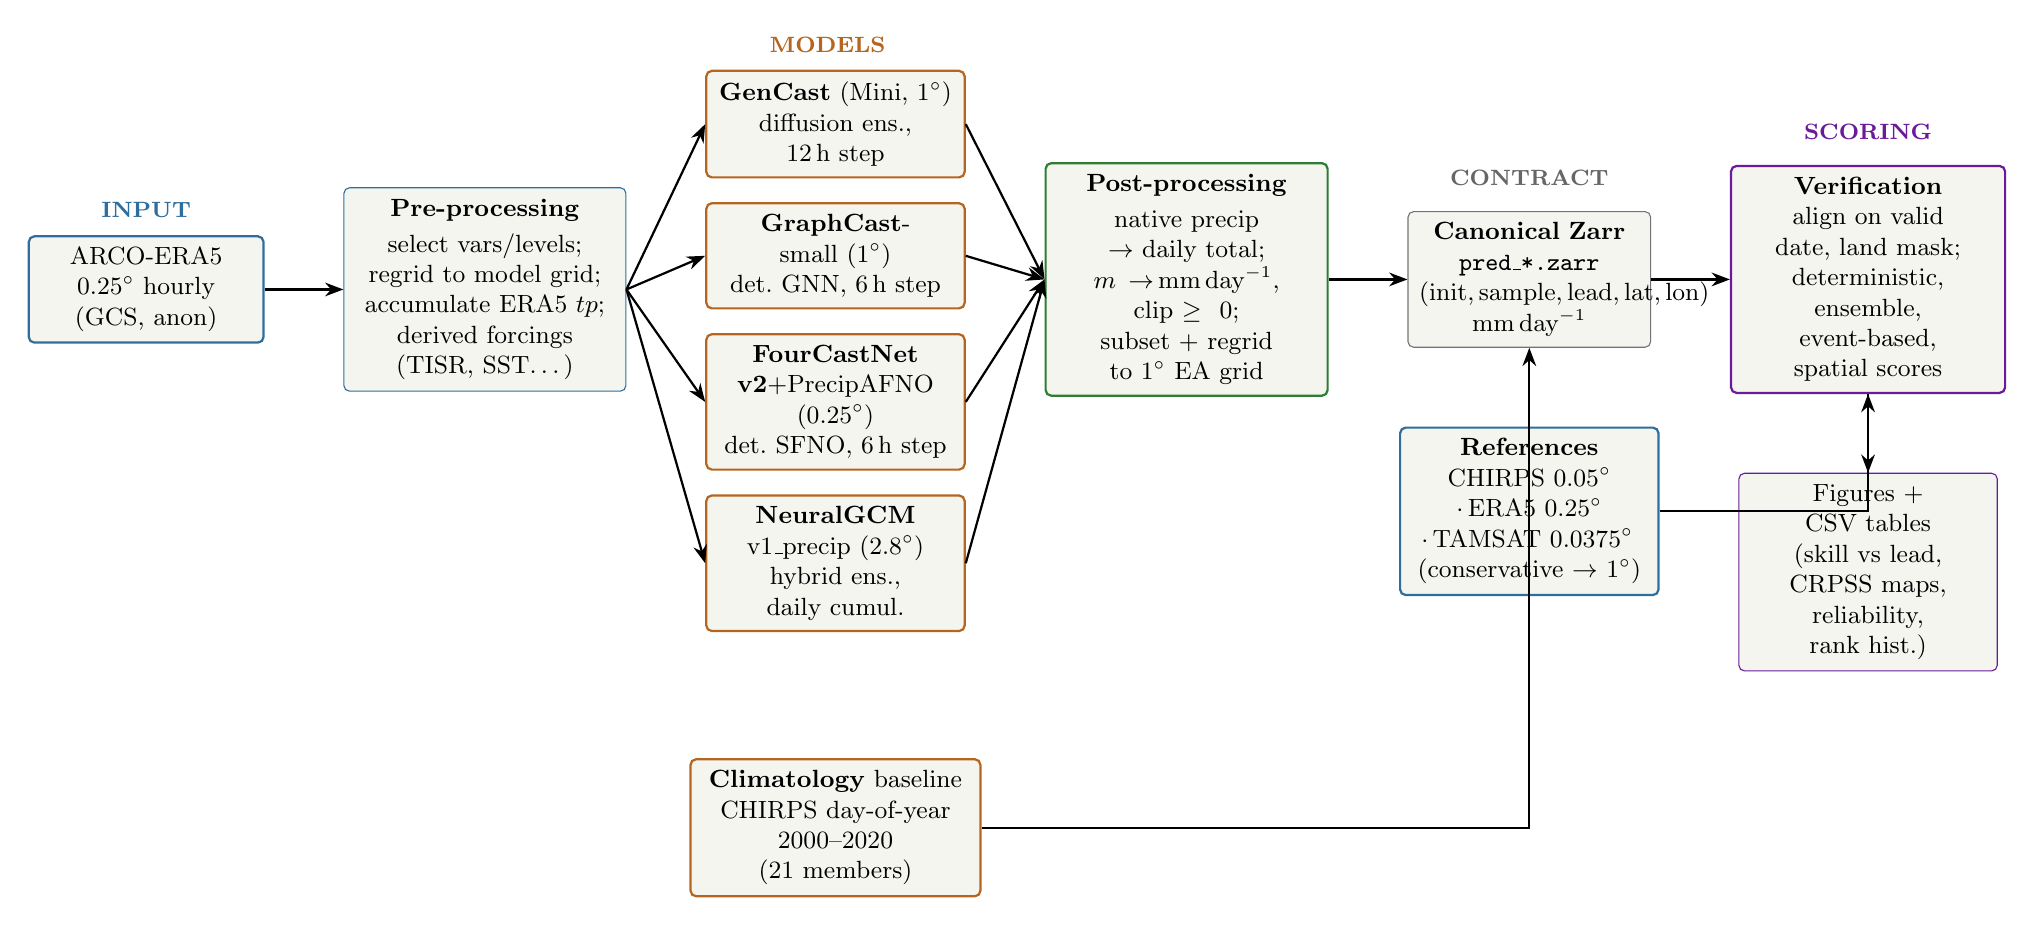
\begin{tikzpicture}[
    font=\small,
    >=Stealth,
    node distance=6mm,
    box/.style={rounded corners=2pt, draw, fill=cBox, align=center,
                inner sep=4pt, minimum height=8mm, text width=27mm},
    src/.style={box, draw=cData, thick, text=black},
    mdl/.style={box, draw=cModel, thick},
    post/.style={box, draw=cPost, thick},
    ver/.style={box, draw=cVerif, thick},
    lbl/.style={midway, font=\scriptsize\itshape, text=black!60},
    stage/.style={font=\bfseries\footnotesize}
]

% --- input ---
\node[src] (era5) {ARCO-ERA5\\ \ang{0.25} hourly\\ (GCS, anon)};

% --- preprocessing column ---
\node[box, draw=cData, right=10mm of era5, text width=33mm] (pre)
  {\textbf{Pre-processing}\\[2pt]
   select vars/levels;\\ regrid to model grid;\\ accumulate ERA5 $tp$;\\
   derived forcings (TISR, SST\ldots)};

% --- models ---
\node[mdl, right=10mm of pre, yshift=21mm, text width=30mm] (gc)
   {\textbf{GenCast} (Mini, \ang{1})\\ diffusion ens., 12\,h step};
\node[mdl, below=3mm of gc, text width=30mm] (grf)
   {\textbf{GraphCast}-small (\ang{1})\\ det.\ GNN, 6\,h step};
\node[mdl, below=3mm of grf, text width=30mm] (fcn)
   {\textbf{FourCastNet v2}+PrecipAFNO (\ang{0.25})\\ det.\ SFNO, 6\,h step};
\node[mdl, below=3mm of fcn, text width=30mm] (ngcm)
   {\textbf{NeuralGCM} v1\_precip (\ang{2.8})\\ hybrid ens., daily cumul.};

% --- postprocessing ---
\node[post, right=10mm of grf, yshift=-3mm, text width=33mm] (post)
  {\textbf{Post-processing}\\[2pt]
   native precip $\to$ daily total;\\ $m\to$\,\mmday, clip $\ge0$;\\
   subset + regrid to \ang{1} EA grid};

% --- canonical store ---
\node[box, draw=black!55, right=10mm of post, text width=28mm] (zarr)
  {\textbf{Canonical Zarr}\\ \code{pred\_*.zarr}\\
   (init,\,sample,\,lead,\,lat,\,lon)\\ \mmday};

% --- climatology branch ---
\node[mdl, below=16mm of ngcm, text width=34mm] (clim)
  {\textbf{Climatology} baseline\\ CHIRPS day-of-year\\ 2000--2020 (21 members)};

% --- references ---
\node[src, below=10mm of zarr, text width=30mm] (obs)
  {\textbf{References}\\ CHIRPS \ang{0.05} $\!\cdot\!$ ERA5 \ang{0.25}\\
   $\!\cdot\!$ TAMSAT \ang{0.0375}\\ (conservative $\to$ \ang{1})};

% --- verification ---
\node[ver, right=10mm of zarr, text width=32mm] (ver)
  {\textbf{Verification}\\ align on valid date, land mask;\\
   deterministic, ensemble,\\ event-based, spatial scores};

% --- outputs ---
\node[box, draw=cVerif, below=10mm of ver, text width=30mm] (out)
  {Figures + CSV tables\\ (skill vs lead, CRPSS maps,\\ reliability, rank hist.)};

% --- arrows ---
\draw[->, thick] (era5) -- (pre);
\draw[->, thick] (pre.east) -- (gc.west);
\draw[->, thick] (pre.east) -- (grf.west);
\draw[->, thick] (pre.east) -- (fcn.west);
\draw[->, thick] (pre.east) -- (ngcm.west);
\draw[->, thick] (gc.east)  -- (post.west);
\draw[->, thick] (grf.east) -- (post.west);
\draw[->, thick] (fcn.east) -- (post.west);
\draw[->, thick] (ngcm.east)-- (post.west);
\draw[->, thick] (post) -- (zarr);
\draw[->, thick] (clim.east) -| (zarr.south);
\draw[->, thick] (zarr) -- (ver);
\draw[->, thick] (obs.east) -| (ver.south);
\draw[->, thick] (ver) -- (out);

% stage labels
\node[stage, above=1mm of era5, text=cData] {INPUT};
\node[stage, above=1mm of gc, text=cModel, xshift=-1mm] {MODELS};
\node[stage, above=2mm of zarr, text=black!60] {CONTRACT};
\node[stage, above=2mm of ver, text=cVerif] {SCORING};

\end{tikzpicture}%
}
\caption{End-to-end data flow. ERA5 analyses are pre-processed per model,
integrated forward, then post-processed to a common daily-total field on the
\ang{1} East Africa grid and written to per-initialization Zarr stores (the
model-agnostic ``contract''). The climatology baseline enters the same contract
directly from CHIRPS. Verification aligns each forecast with three rainfall
references on the valid date and emits figures and tables.}
\label{fig:flow}
\end{figure}
% ---------------------------------------------------------------------------

% ===========================================================================
\section{Models and their motivation}
% ===========================================================================

Four machine-learning forecast systems are benchmarked against a climatological
baseline (Table~\ref{tab:models}). The four are chosen to span the distinct
\emph{architectural families} of data-driven weather prediction, so that
conclusions are not specific to one design.

\begin{table}[t]
\centering
\small
\begin{tabular}{@{}p{2.5cm}p{3.0cm}p{2.3cm}p{3.0cm}c@{}}
\toprule
\textbf{Model} & \textbf{Family} & \textbf{Native res.} &
\textbf{Native precip $\to$ daily} & \textbf{Members}\\
\midrule
GenCast (Mini) & Diffusion generative ensemble & \ang{1}, 13 lev. &
  12\,h accum., sum $2\times$12\,h & 10\\
GraphCast-small & Deterministic GNN & \ang{1}, 13 lev., mesh 2$\to$5 &
  6\,h accum., sum $4\times$6\,h & 1\\
FourCastNet v2 & Spherical Fourier neural operator & \ang{0.25} &
  6\,h accum.\ (PrecipAFNO), sum $4\times$6\,h & 1\\
NeuralGCM & Hybrid physics-ML & $\sim$\ang{2.8} ($128{\times}64$) &
  daily cumulative, de-accumulate & 10\\
Climatology & CHIRPS day-of-year & \ang{1} & observed (no rollout) & 21\\
\bottomrule
\end{tabular}
\caption{Benchmarked systems and how each native precipitation output becomes a
00--00\,UTC daily total. The exact checkpoints are given in
Section~\ref{sec:models-detail}.}
\label{tab:models}
\end{table}

\paragraph{GenCast (diffusion ensemble).} A conditional-diffusion generative
model that samples full weather trajectories, and the first ML system to
outperform the leading operational ensemble (ECMWF~ENS) on a majority of
targets. It is the natural headline for a rainfall benchmark because it produces
a calibrated \emph{ensemble} --- uncertainty matters as much as the central
estimate for precipitation --- and it emits precipitation natively. We draw a
10-member ensemble per initialization from distinct random seeds.

\paragraph{GraphCast (deterministic GNN).} A message-passing graph neural
network run autoregressively; it outperformed the operational deterministic
model (HRES) on most variables at a fraction of the cost and is the most widely
used deterministic AI-NWP baseline. It anchors the deterministic end of the
comparison.

\paragraph{FourCastNet v2 (neural operator).} A spherical Fourier neural
operator (SFNO), an operator-learning architecture distinct from both the
message-passing GNN and the diffusion model, included specifically to guard
against architecture-specific conclusions. It has no native precipitation, so
rainfall is obtained from the separate PrecipitationAFNO diagnostic (see
Section~\ref{sec:models-detail}).

\paragraph{NeuralGCM (hybrid physics-ML).} A differentiable atmospheric
dynamical core coupled to learned sub-grid physics --- a fundamentally different
design point from the purely data-driven emulators above. Its ensemble spread
arises from \emph{stochastic physics} (a native source of dispersion rather than
input perturbations), and the \code{v1\_precip} checkpoint predicts
precipitation directly. Its coarse resolution makes it a clean test of whether
physical constraints compensate for reduced spatial detail. We draw 10 members.

\paragraph{Climatology (baseline).} The indispensable no-skill reference,
constructed from the day-of-year distribution of CHIRPS observations over
2000--2020 (21 members, one per reference year). It is strictly out-of-sample
with respect to the 2024 evaluation and shares the exact spatial coverage of the
verification data; beating a well-constructed day-of-year climatology for
tropical rainfall is a non-trivial bar, which is why it is the reference against
which skill (CRPSS) is defined.

% ===========================================================================
\section{Per-model pre- and post-processing for the 2024 rainfall forecasts}
\label{sec:models-detail}
% ===========================================================================

All learned models are initialised from ARCO-ERA5 and their precipitation output
is converted to a 00--00\,UTC daily total on the common \ang{1} grid. The two
processing ends differ per model because the native output cadence differs; the
target is always the accumulation over the 24\,h window ending at
$t+\ell$~days.

% ---------------------------------------------------------------------------
\subsection{GenCast --- Mini \ang{1} checkpoint}
\textbf{Checkpoint.} \code{gs://dm\_graphcast/gencast/params/} (the ``Mini''
\ang{1}, 13-level checkpoint is auto-selected).\\
\textbf{Pre-processing.} Two input states at $t_0$ and $t_0{+}12$\,h are built
from ERA5: six pressure-level fields (temperature, geopotential, $u$, $v$,
vertical velocity, specific humidity) on 13 levels and five surface fields
(2\,m temperature, SST, 10\,m $u/v$, MSLP), bilinearly interpolated to a global
\ang{1} grid; precipitation is formed by summing hourly ERA5 \code{total\_%
precipitation} over the 12\,h window ending at each stamp. Static fields
(land--sea mask, surface geopotential) and derived solar/temporal forcings are
added via \code{graphcast.data\_utils}.\\
\textbf{Inference.} \code{chunked\_prediction\_generator\_multiple\_runs} with
\code{num\_samples}${=}10$ (per-member RNG via \code{jax.random.fold\_in}),
12\,h autoregressive steps to the maximum lead.\\
\textbf{Post-processing.} The native \code{total\_precipitation\_12hr} (metres)
for lead $L$ is the sum of the steps ending at $(2L{-}1)\,{\cdot}\,12$\,h and
$2L\,{\cdot}\,12$\,h; multiplied by 1000 (m$\to$mm), clipped at zero, subset to
the EA box and bilinearly interpolated to the \ang{1} grid.

% ---------------------------------------------------------------------------
\subsection{GraphCast --- small \ang{1} checkpoint}
\textbf{Checkpoint.} \code{GraphCast\_small --- ERA5 1979--2015 --- resolution
1.0 --- pressure levels 13 --- mesh 2to5 --- precipitation input and output}.\\
\textbf{Pre-processing.} Two input frames at $t_0{-}6$\,h and $t_0$, the same
pressure-level and surface fields as above (MSLP in place of SST), 6\,h
accumulated precipitation, static fields, and forcings comprising day/year
progress and top-of-atmosphere incident solar radiation
(\code{add\_tisr\_var}).\\
\textbf{Inference.} \code{rollout.chunked\_prediction} (deterministic;
\code{rng}${=}$\code{PRNGKey(0)}), 6\,h autoregressive steps.\\
\textbf{Post-processing.} With native 6\,h accumulation there are four steps per
day; the daily total for lead $L$ is the sum of the steps ending at
$(L{-}1)\,{\cdot}\,24 + s\,{\cdot}\,6$\,h for $s\in\{1,2,3,4\}$ ($=24$\,h),
converted to \mmday, clipped, subset and interpolated to the \ang{1} grid,
stored with \code{sample}${=}1$.

% ---------------------------------------------------------------------------
\subsection{FourCastNet v2 --- SFNO + PrecipitationAFNO}
\textbf{Checkpoints.} \code{e2mip://fcnv2\_sm} (SFNO backbone) and
\code{PrecipitationAFNO} diagnostic, via NVIDIA \code{earth2mip}.\\
\textbf{Pre-processing.} A single initial-condition tensor
$(1,1,73,721,1440)$ is assembled from ARCO at $t_0$; earth2mip channel names are
mapped to ARCO variables, and relative-humidity channels (absent from ARCO) are
computed from specific humidity and temperature via the Tetens formula. The ARCO
$721\times1440$ grid matches the SFNO grid exactly, so no interpolation is
needed on input.\\
\textbf{Inference.} The \code{earth2mip} time loop is stepped at 6\,h; the $t{=}0$
yield (the IC itself) is skipped. At each forecast step the 20 channels required
by PrecipitationAFNO are sliced (dropping the south-pole row, $[:720]$) and
passed through the diagnostic to yield 6\,h accumulated precipitation
(metres). Deterministic.\\
\textbf{Post-processing.} Four 6\,h steps are summed per lead day, converted to
\mmday\ and clipped; the descending SFNO latitude axis is flipped to ascending,
then subset and bilinearly interpolated to the \ang{1} grid;
\code{sample}${=}1$.

% ---------------------------------------------------------------------------
\subsection{NeuralGCM --- v1\_precip stochastic \ang{2.8}}
\textbf{Checkpoint.} \code{gs://neuralgcm/models/v1\_precip/%
stochastic\_precip\_2\_8\_deg.pkl} (the only precipitation-emitting checkpoint;
stochastic-only, \ang{2.8}).\\
\textbf{Pre-processing.} The model's required input and forcing variables are
read from ARCO at the initialization time (and along the horizon, 6-hourly, for
prescribed SST/sea-ice) on 37 levels, conservatively regridded from ARCO's
\ang{0.25} grid to the model's $128\times64$ Gaussian grid, with ocean NaNs
filled by nearest neighbour.\\
\textbf{Inference.} For each of 10 members the state is encoded with a distinct
JAX RNG key and unrolled with \code{steps}${=}L_{\max}$,
\code{timedelta}${=}24$\,h and \code{start\_with\_input=False}; SST and sea-ice
forcings over the horizon are prescribed from ERA5 (``perfect forcing'').\\
\textbf{Post-processing.} The native \code{precipitation\_cumulative\_mean} is a
precipitation \emph{depth accumulated from initialization} (metres,
monotonically increasing). The per-day total is recovered by consecutive
differencing --- day~1 is the value itself, day~$k$ is
$C(k)-C(k-1)$ --- then $\times1000$, clipped, subset (with a wider buffer given
the coarse grid) and bilinearly interpolated to the \ang{1} grid; the model's
$(\text{lon},\text{lat})$ axes are transposed to the canonical
$(\text{lat},\text{lon})$. Sample values were validated against CHIRPS
($\approx 2.3/4.4/5.1$~\mmday\ at $+1/2/3$\,d for a March~2024 initialization).

% ---------------------------------------------------------------------------
\subsection{Climatology baseline}
For initialization $t$ and lead $L$ the ``forecast'' is the set of CHIRPS
observations sharing the day-of-year of the valid date $t{+}L$, drawn from each
reference year 2000--2020 (21 members; day-of-year~366 falls back to~365).
CHIRPS is already in \mmday\ and is conservatively regridded once to the \ang{1}
grid, so no accumulation or unit conversion is applied. This yields a genuine
probabilistic baseline with the same spatial coverage as the verification data.

\paragraph{Common post-processing invariants.} Every learned model:
(i)~forms daily totals from its native cadence as above;
(ii)~converts metres to \mmday\ and clips negatives to zero;
(iii)~subsets to a box slightly larger than the EA domain and bilinearly
interpolates to \code{config.lat\_vals}${\times}$\code{config.lon\_vals};
(iv)~writes the canonical \code{total\_precipitation} array. This makes the
prediction stores byte-compatible for verification regardless of the source
model's grid, cadence, or ensemble size.

% ===========================================================================
\section{Reference observations}
% ===========================================================================

To ensure conclusions are not artefacts of a single product, forecasts are
verified against three independent rainfall references, each conservatively
(area-weighted, xESMF) regridded from its native resolution to the common
\ang{1} grid: \textbf{CHIRPS~v2.0} (\ang{0.05}, blended gauge--satellite; the
primary reference and the source of the climatology), \textbf{ERA5} total
precipitation (\ang{0.25} reanalysis, hourly accumulations summed to daily
totals), and \textbf{TAMSAT~v3.1} (\ang{0.0375}, satellite estimate). Reporting
against all three characterises sensitivity to observational uncertainty over a
gauge-sparse region.

% ===========================================================================
\section{Experimental setup: what has been done in this codebase}
\label{sec:metrics}
% ===========================================================================

\paragraph{Forecast generation (complete).} All four learned models and the
climatology baseline are implemented as adapters behind the common interface and
have been run to produce \code{total\_precipitation} for 2024 initializations at
leads $\{1,3,5,7\}$ on the \ang{1} EA grid. GenCast, GraphCast and
FourCastNet~v2 run in a single JAX\,$+$\,PyTorch/\code{earth2mip} environment;
NeuralGCM runs in a \emph{dedicated} environment (its JAX/\code{dinosaur} stack
is incompatible with the graphcast environment) and is launched separately via
\code{run\_neuralgcm.sh}. Each model is assigned its own GPU, and each
initialization is an independent, resumable output file.

\paragraph{Verification metrics (implemented in \code{run\_verification.py}).}
The scoring stage aligns forecasts with each reference on the valid date over
land cells and computes:
\begin{itemize}[nosep,leftmargin=1.4em]
  \item \textbf{Deterministic} (ensemble mean or single forecast): bias, MAE,
        RMSE, and spatial/temporal correlation.
  \item \textbf{Event-based} at exceedance thresholds $\{1,5,10,20\}$~\mmday:
        contingency-table scores --- probability of detection, false-alarm
        ratio, critical success index, and frequency bias.
  \item \textbf{Ensemble/probabilistic}: fair (bias-corrected) CRPS, ensemble
        spread and spread--skill ratio, Brier score, nominal $50/80/90\%$
        interval coverage and width, Talagrand rank histograms (with
        Hamill randomisation of ties to handle the many exact zeros in
        rainfall), reliability diagrams (fixed and local-percentile thresholds)
        with Wilson confidence intervals and the expected calibration error.
  \item \textbf{Skill vs.\ climatology}: the CRPS skill score
        $\text{CRPSS}=1-\text{CRPS}_{\text{model}}/\text{CRPS}_{\text{clim}}$,
        as scalars per lead and as per-cell maps (with hyper-arid cells masked).
  \item \textbf{Spatial and temporal diagnostics}: per-cell bias/RMSE maps,
        area-mean time series against all three references, and rolling
        bias/MAE (and, for the ensemble, CRPS/spread/SSR) skill curves.
\end{itemize}
Outputs are written as PNG figures and CSV tables. Companion scripts
(\code{crpss\_skill\_maps*.py}, \code{acc\_lead\_curves.py},
\code{ssr\_lead\_curves.py}, \code{ssr\_zonal\_profile.py}) reproduce specific
figures from the same prediction stores.

\paragraph{Current scope and caveats (grounded in the code as it stands).}
\begin{itemize}[nosep,leftmargin=1.4em]
  \item \emph{Evaluation window.} Forecasts exist for the full year, but the
        verification driver and the standalone skill scripts currently
        \emph{default} to the March--May (MAM) long-rains window
        (\code{--start 2024-03-01 --end 2024-05-31}); the window is a command-line
        argument and can be set to the full year.
  \item \emph{Model coverage in scoring.} The verification driver's default
        model set and its plotting metadata cover GenCast, GraphCast and
        FourCastNet~v2, with climatology loaded as an optional baseline for
        CRPSS. NeuralGCM is inference-complete and written in the canonical
        format, but its integration into the verification driver's
        labels/palette is still pending.
  \item \emph{Ensemble calibration diagnostics.} Rank histograms, reliability,
        interval coverage and the Brier/CRPS ensemble tables are currently
        computed for the GenCast ensemble specifically; extending them to the
        NeuralGCM ensemble is a natural next step.
  \item \emph{Verification resolution.} All scoring is at \ang{1}. The finer
        native resolution of FourCastNet~v2 (\ang{0.25}) and the coarser
        resolution of NeuralGCM (\ang{2.8}) are both mapped to this grid, so the
        comparison is fair but does not reward or penalise sub-\ang{1}
        structure.
\end{itemize}

\paragraph{Reproducibility.} The benchmark is a single pipeline built on xarray,
Zarr, xESMF and \code{properscoring}/\code{scores}. All inputs are public
(checkpoints and ERA5 from anonymous GCS; CHIRPS/ERA5/TAMSAT downloaded and
cached on first use), inference and verification are separate stages, and every
forecast is a self-describing per-initialization file, so results can be
regenerated or re-scored incrementally.

\end{document}
